В силу проблем возникающих при смешении грамматик языков и возникающих при этом shift/reduce или reduce/reduce конфликтов некоторые правила для конструкций реализованы не в полном объеме.
\begin{itemize}

\item Добавлено ключевое слово {\it match} и теперь оно не может использоваться в качестве идентификатора.

\item Можно использовать другой стиль стрелок («->» вместо «=>») в pattern matching, но в таком случае не работает {\it when} (одна из дополнительных функций).

\item Можно писать pattern matching в стиле \OCaml{}.%, но тогда после стрелки может идти только единичное выражение, а не их последовательность.%\footnote[1]{Однако эта проблема легко решается заключением последовательности в \{\}. }

\item Можно писать условие и тело цикла в стиле \OCaml{}.

\item Можно использовать разделитель <<;>> вместо <<,>> в объявлении record.

\item Можно объявлять модули в стиле \OCaml{}.

\item Можно писать {\it if} с {\it then}.

\end{itemize}

Так же добавлены предупреждения (warning) для всех синтаксических конструкций перечисленных выше. И реализовано быстрое исправление кода (<<Quick fix>>) в OCaml-LSP, которое заменяет {\it match with} и {\it struct end} на подходящие языку Reason ключевые слова.
\begin{figure}[h]
\begin{subfigure}{0.5\textwidth}
	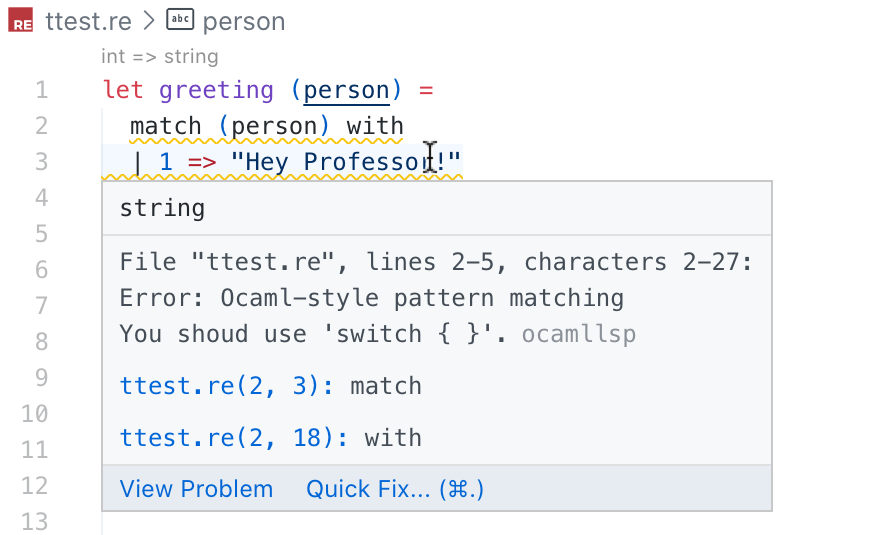
\includegraphics[width=\linewidth]{screenshots/05.png}
\end{subfigure}
\begin{subfigure}{0.5\textwidth}
	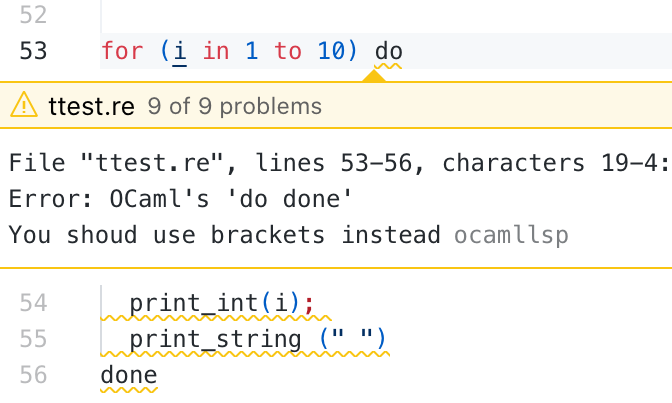
\includegraphics[width=\linewidth]{screenshots/06.png}
\end{subfigure}
\caption{Примеры}
\end{figure}

\newpage
Для симметричной задачи, для OCaml реализованы предупреждения в OCaml-LSP для следующих конструкций из Reason: определение модуля, pattern matching (при этом стрелки должны быть из OCaml), запятые в record. Для этих конструкций реализованы соответствующие быстрые исправления в OCaml-LSP:
\begin{itemize}

\item Замена {\it \{ \}} на {\it struct end}.

\item Замена {\it switch \{ \}} на {\it match with}.

\item Замена всех <<,>> на <<;>> в объявлении record.

\end{itemize}

\begin{figure}[h]
\begin{subfigure}{0.5\textwidth}
	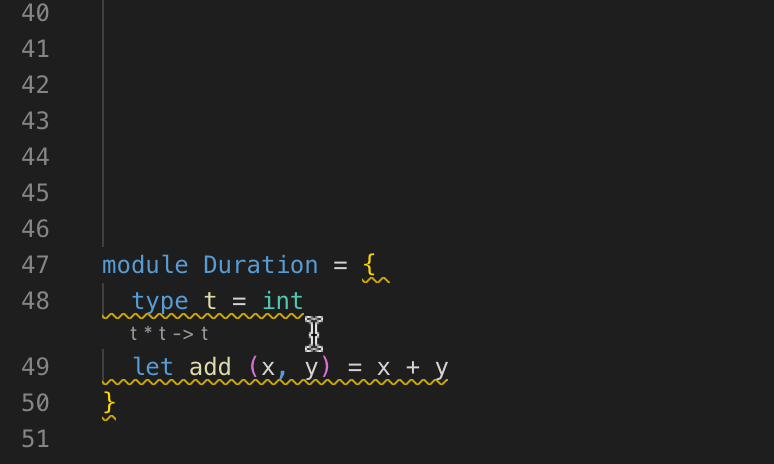
\includegraphics[width=\linewidth]{screenshots/01.png}
\end{subfigure}
\begin{subfigure}{0.5\textwidth}
	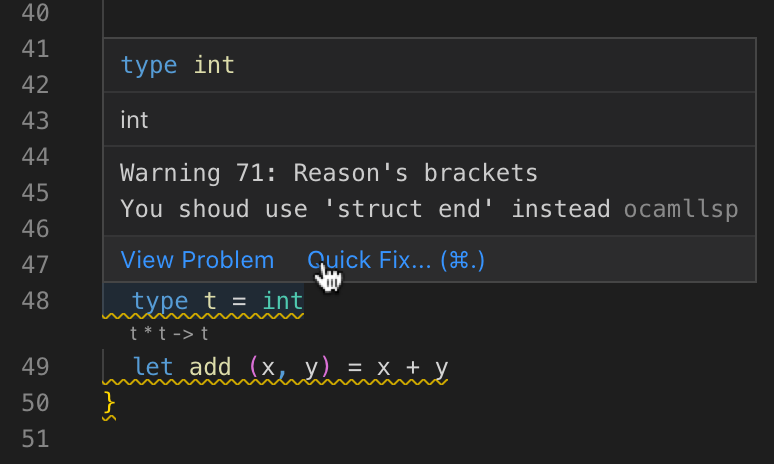
\includegraphics[width=\linewidth]{screenshots/02.png}
\end{subfigure}
\newline
\begin{subfigure}{0.5\textwidth}
	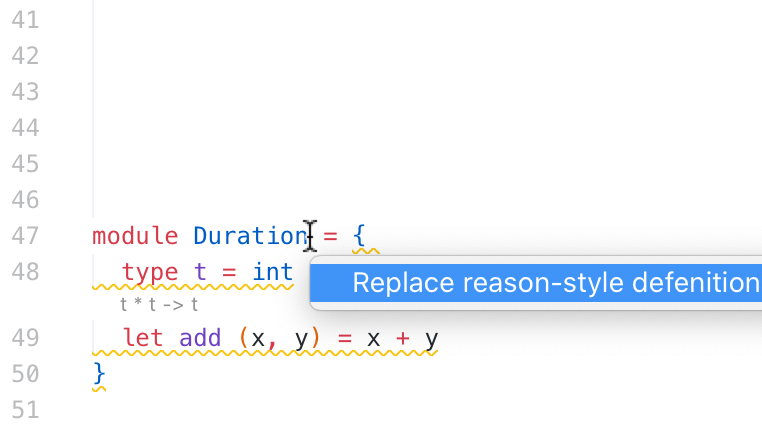
\includegraphics[width=\linewidth]{screenshots/03.png}
\end{subfigure}
\begin{subfigure}{0.5\textwidth}
	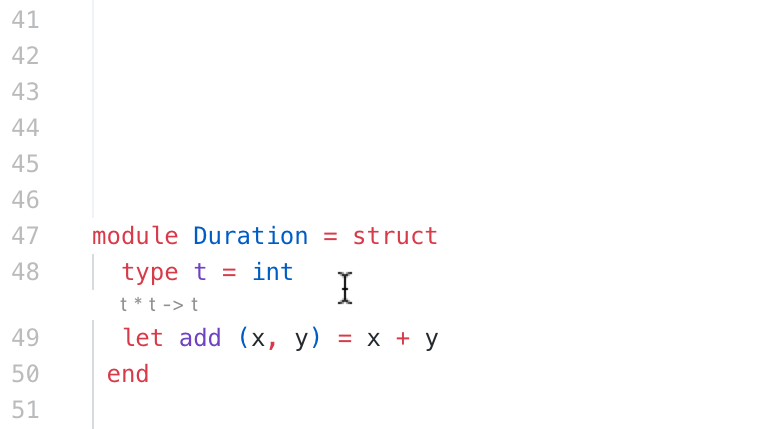
\includegraphics[width=\linewidth]{screenshots/04.png}
\end{subfigure}
\caption{Исправление кода OCaml}
	\label{fix}%fig3
\end{figure}

Результаты проделанной работы можно наблюдать в соответсвующих репозиториях. Ссылки на списки коммитов Reason\footnote[1]{ \url{https://github.com/pereb4ik/reason/commits?author=pereb4ik} },
OCaml-LSP\footnote[2]{ \url{https://github.com/pereb4ik/ocaml-lsp/commits?author=pereb4ik} },
merlin\footnote[3]{ \url{https://github.com/pereb4ik/merlin/commits/lsp?author=pereb4ik} }.
\newpage

\subsection{Установка}
Необходимая версия OCaml~--- 4.13.1/4.13.
 
Reason устанавливается через:
% ":" not italic, i don't know
\lstset{emph={https}, emphstyle={\itshape \small} }
\lstset{basicstyle=\ttfamily}
\begin{example}
\begin{lstlisting}[frame=single,language=C]
opam pin add reason https://github.com/pereb4ik/reason.git
\end{lstlisting}
\caption{}
\end{example}
При необходимости так же rtop:
\begin{example}
\begin{lstlisting}[frame=single,language=C]
opam pin add rtop https://github.com/pereb4ik/reason.git
\end{lstlisting}
\caption{}
\end{example}
Для тестирования функций IDE, умной замены кода <<Quick fix>> понадобится Visual Studio Code (хотя ocaml-lsp можно использовать с другими редакторами) с расширением OCaml Platform\footnote[4]{ \url{https://marketplace.visualstudio.com/items?itemName=ocamllabs.ocaml-platform} } от OCaml Labs. И пакет ocaml-lsp <<нашей>> версии:
\begin{example}
\begin{lstlisting}[frame=single,
language=C,
% fix stupid bug with bad "-" in copying from pdf
literate={-}{-}1
]
opam pin add ocaml-lsp-server https://github.com/pereb4ik/ocaml-lsp.git
\end{lstlisting}
\caption{}
\end{example}